\section{Methods}

This section describes in detail the approach to the classification problem
in documents that contain handwritten text as well as handwritten illustrations.

As in the case of Scene Text Detection/Recognition, it is effective to separate Text Detection
and Text Recognition and treat them as different problems.
Furthermore, it is possible to record the written area due to the characteristics of the electronic tablet,
so using a simple heuristic on the trajectory data eliminates the need to actually perform text detection.
The role of this step, namely "Region of Interest Detection" step is to reduce the size of data
passed to the subsequent processing and suppress the increase in the amount of calculation.

In general, electronic tablets have severe limitations on computing power, so in this report
I used the heuristic to detect region of interst. Detected regions are then preprocessed
and passed to the text recognition module. In the text recognition module,
two patterns of recognition using CTC and recognition combining
Character Segmentation and Character Recognition were verified.


\subsection{Region of Interest Detection}

\subsection{Recognition}

In text recognition, two models were tried: a model that directly reads the content from the
result of region of interest detection using CTC, and a two-staged approach in which
Character Segmentation and Character Recognition were connected in series.

\subsubsection{CTC}

\subsubsection{Character Segmentation}

\subsubsection{Character Recognition}

It is known that character recognition is sufficiently accurate even if
a simple neural network model is used. Therefore, a small CNN model was designed
in consideration of the amount of calculation.

\subsection{Auto-Complete}

\subsection{Dataset}

% TODO: add footnotes
Handwritten character recognition and handwritten sentence recognition are
fields that have been studied for a long time, so there are many data sets,
but these are often provided in different formats, and there is some difficulty
in eliminating differences between formats and using them for training dataset.

I therefore took an approach to create a composite dataset by
embedding a combination of existing handwritten-like fonts and
randomly selected English words in the image.
Figure \ref{fig:generated_image} shows an example of training data generated with this method.

\begin{figure}
    \centering
    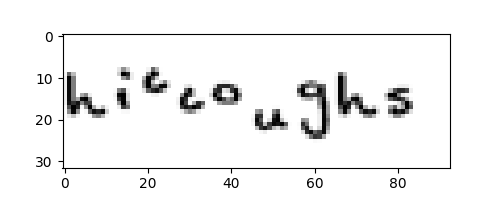
\includegraphics[width=\linewidth]{images/generated_image.png}
    \caption{Generated image using handwritten-like fonts}
    \label{fig:generated_image}
\end{figure}

\subsection{Implementation}


